\title{Midterm - INTD290}
\author{Dr. Jordan Hanson - Whittier College Dept. of Physics and Astronomy}
\date{\today}
\documentclass[10pt]{article}
\usepackage[a4paper, total={18cm, 27cm}]{geometry}
\usepackage{outlines}
\usepackage{hyperref}
\usepackage{graphicx,subfigure}
\begin{document}
\maketitle

\section{How to Submit this Midterm}

\begin{enumerate}
\item Complete your work on this midterm.
\item Scan it into PDF form using a smartphone app, scanner, or digital picture
\item Alternatively you can type up your answers in a separate file, but it still must be a PDF
\item Submit it using the link on Moodle
\end{enumerate}

\section{Maps of The New World}

\begin{figure}[ht]
\centering
	\subfigure[Virreinato 1]{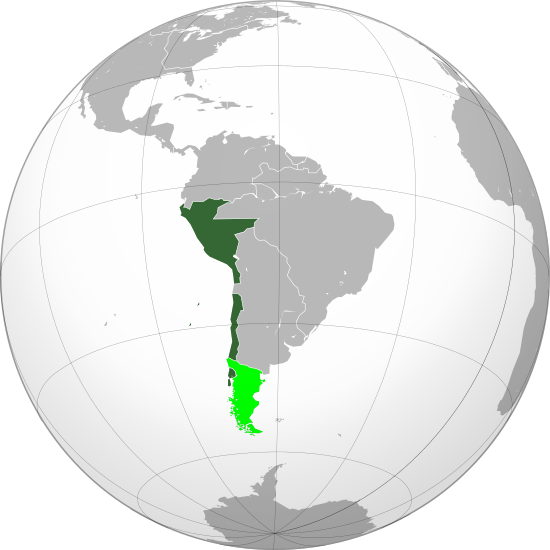
\includegraphics[width=0.2\textwidth]{figures/vice_peru.png}}
	\subfigure[Virreinato 2]{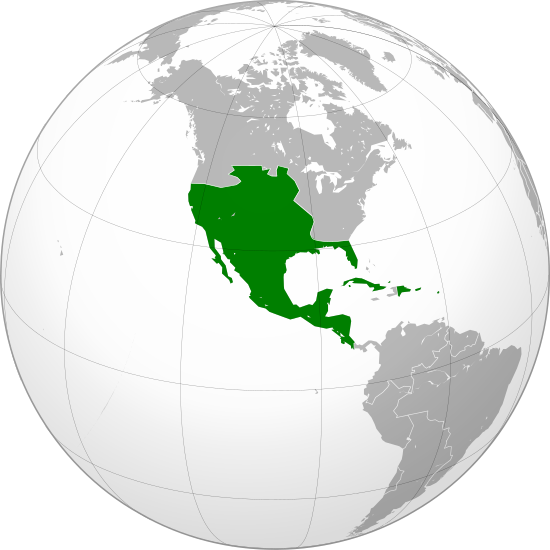
\includegraphics[width=0.2\textwidth]{figures/vice_nuevaespana.png}}
	\subfigure[Virreinato 3]{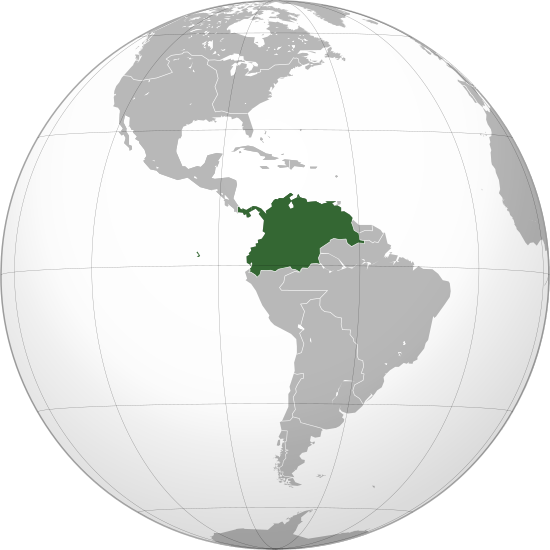
\includegraphics[width=0.2\textwidth]{figures/vice_nuevagranada.png}}
	\subfigure[Virreinato 4]{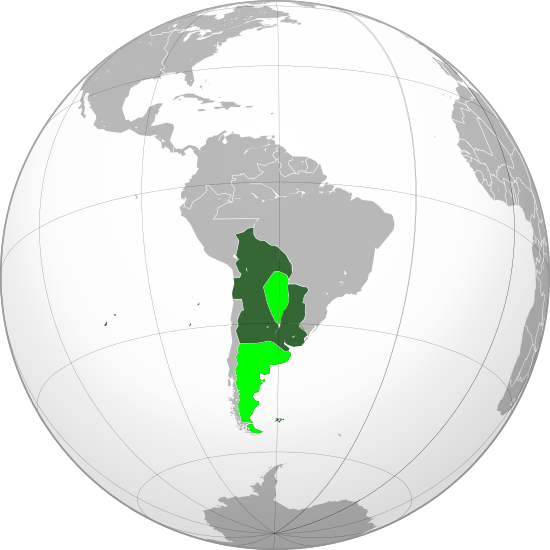
\includegraphics[width=0.2\textwidth]{figures/vice_riodelaplata.png}}
\caption{\label{fig:map1} There were up to four \textit{virreinatos} during the Spanish colonial period of Latin American history.}
\end{figure}

\begin{enumerate}
\item In which of the four \textit{virreinatos} of the Spanish colonial empire (shown in Fig. \ref{fig:map1}) was the \textit{tle huitzilin} classified by the indigenous?
\item Which of the four \textit{virreinatos} excelled at the exportation of rum?
\item Which of the four \textit{virreinatos} was characterized by an indigenous empire that mastered agriculture in the Andean mountains?
\item The low-latitude aurora of 1789 was observed in \textit{which cities?}  In which of the four virreinatos are these cities?  List some other countries in which corresponding observations were made.
\item List some of the locations explored by La Condamine and his Latin American collegues, and cite the virreinato or virreinatos they explored together.
\item The Expedici\'{o}n Bot\'{a}nica of Jos\'{e} Celestino Mutis took place in which virreinato?
\item Jos\'{e} Celestino Mutis took place in which virreinato?  Mutis was the inaugural chair of the department of mathematics at the \textit{Colegio del Rosario}.  In which city is this?
\item In which country is the Pierre Auger Observatory located?  In which virreinato would this country have been in the 18th century?
\end{enumerate}

\clearpage

\section{Asynchronous Activity Review I}

\begin{figure}
\centering
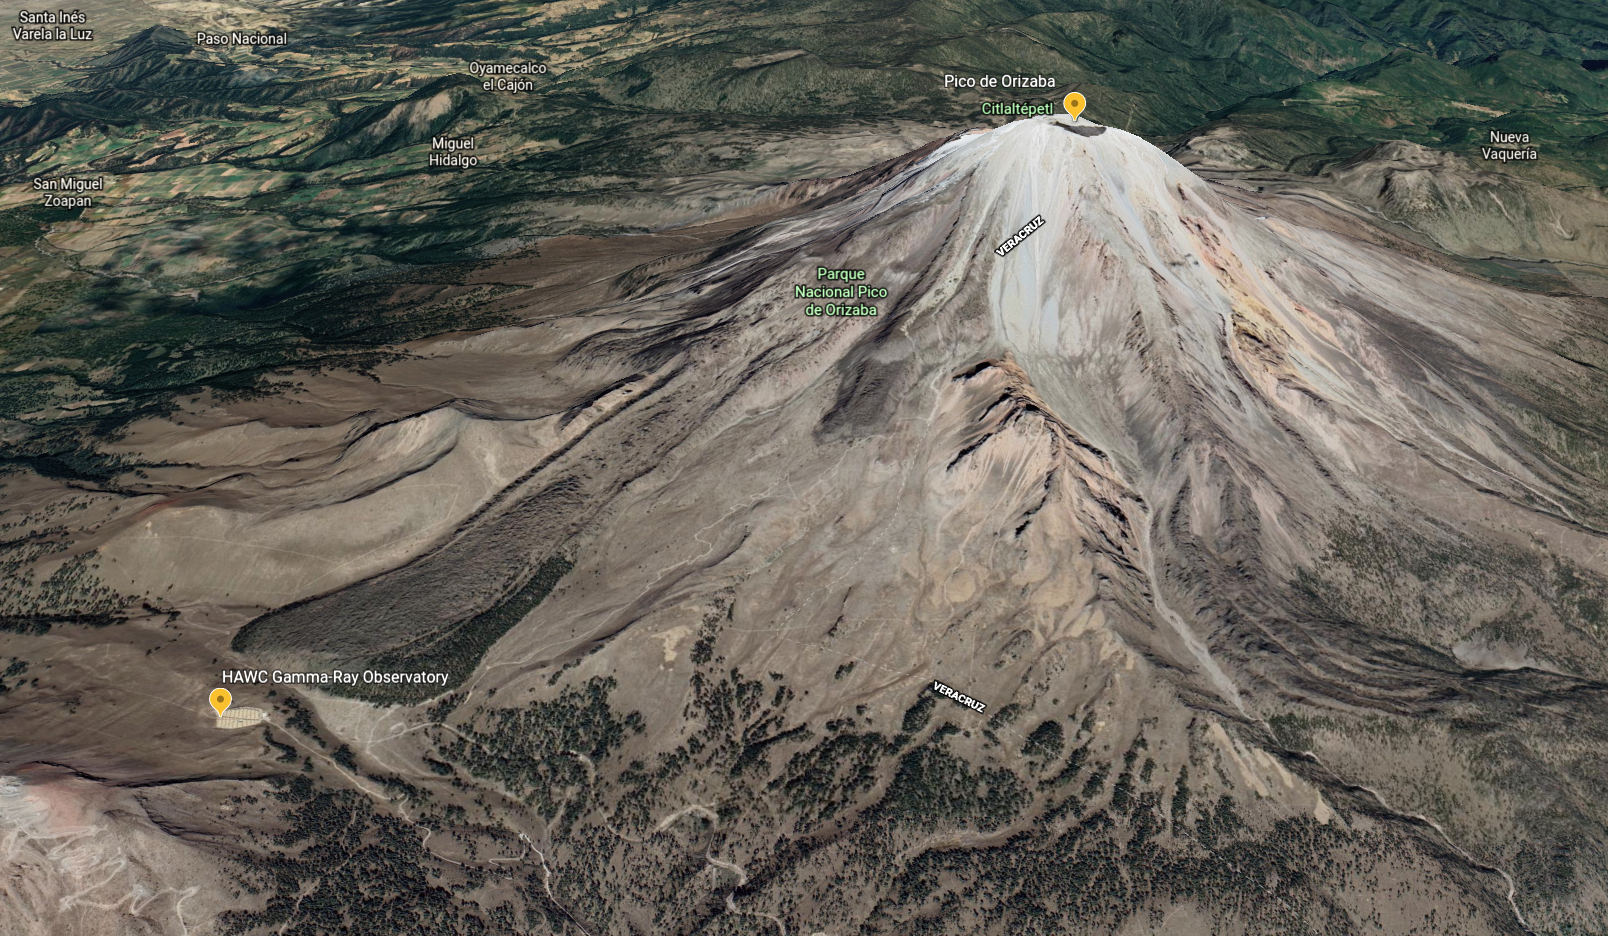
\includegraphics[width=0.45\textwidth]{figures/hawc.png}
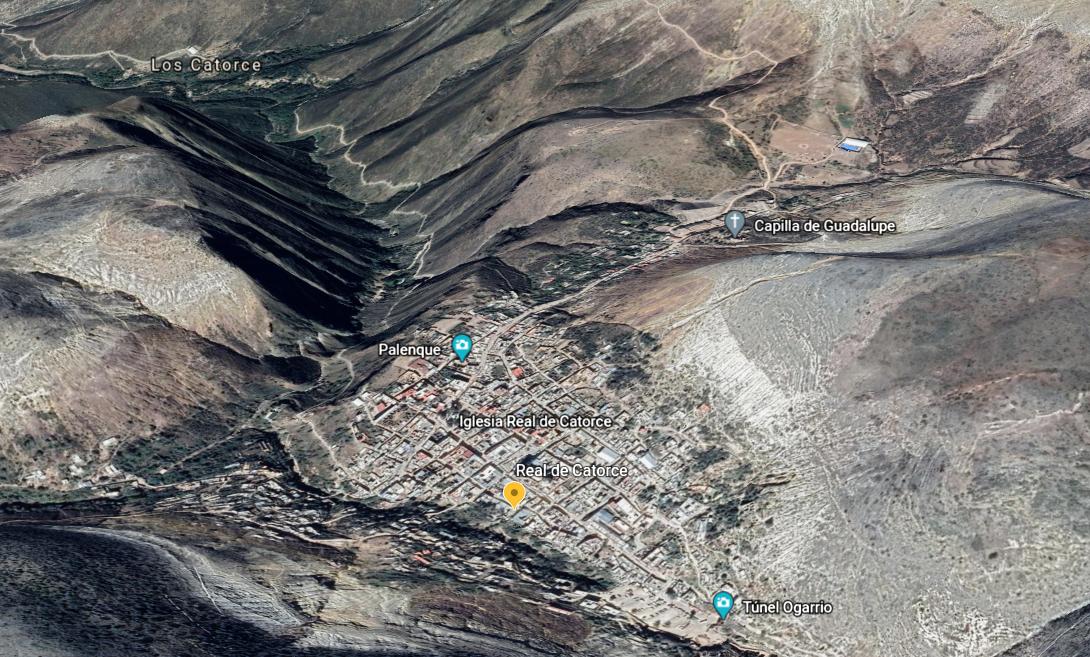
\includegraphics[width=0.45\textwidth]{figures/real.png}
\caption{\label{fig:mines} (Left) A physics detector near Pico de Orizaba in Mexico. (Right) A town in central Mexico.}
\end{figure}

\begin{enumerate}
\item What is the physics detector shown in Fig. \ref{fig:mines} (left)?  Explain in basic terms the purpose of this detector and how it works. \\ \vspace{2cm}
\item What is the significance of Mexican cities as pictured in Fig. \ref{fig:mines} (right), in the context of the development of colleges and the scientific community in 18th century Mexico? \\ \vspace{2cm}
\item What city is being shown in Fig. \ref{fig:mines2}?  In which country is it located, and what was the historical significance of this city for international trade?  Who controlled it?  From where the commodity produced here originate, and how was it shipped to Europe and Africa?
\end{enumerate}

\begin{figure}
\centering
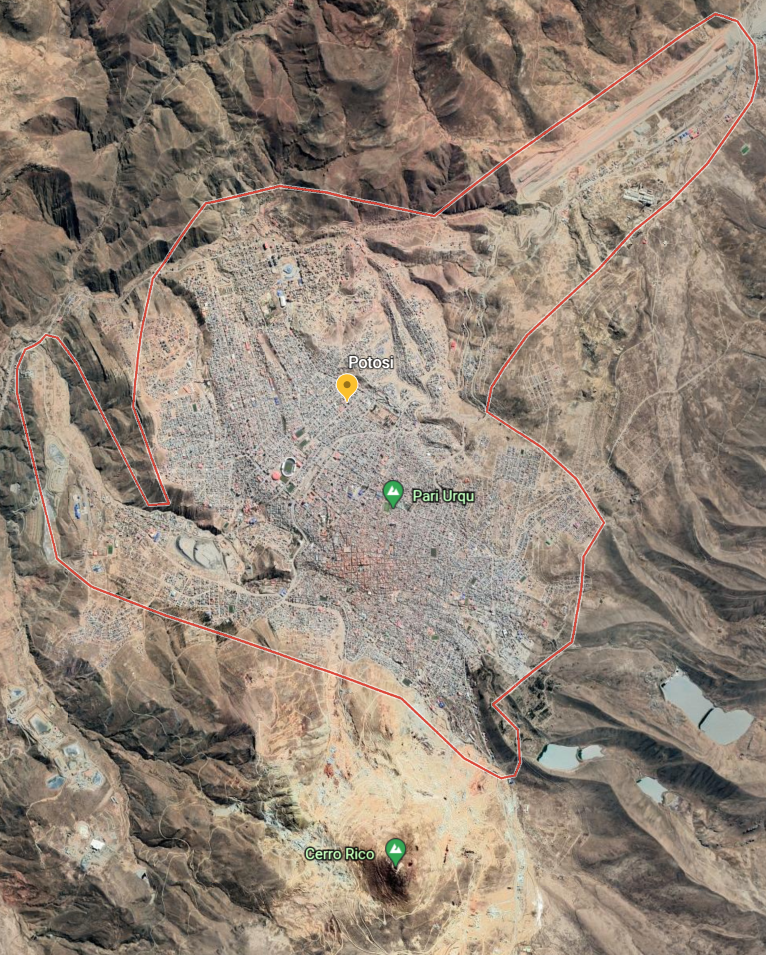
\includegraphics[width=0.33\textwidth]{figures/cerro.png}
\caption{\label{fig:mines2} A historical location in Latin America known for driving a particular economic sector.}
\end{figure}

\clearpage

\section{Asynchronous Activity Review II}

\begin{figure}[hb]
\centering
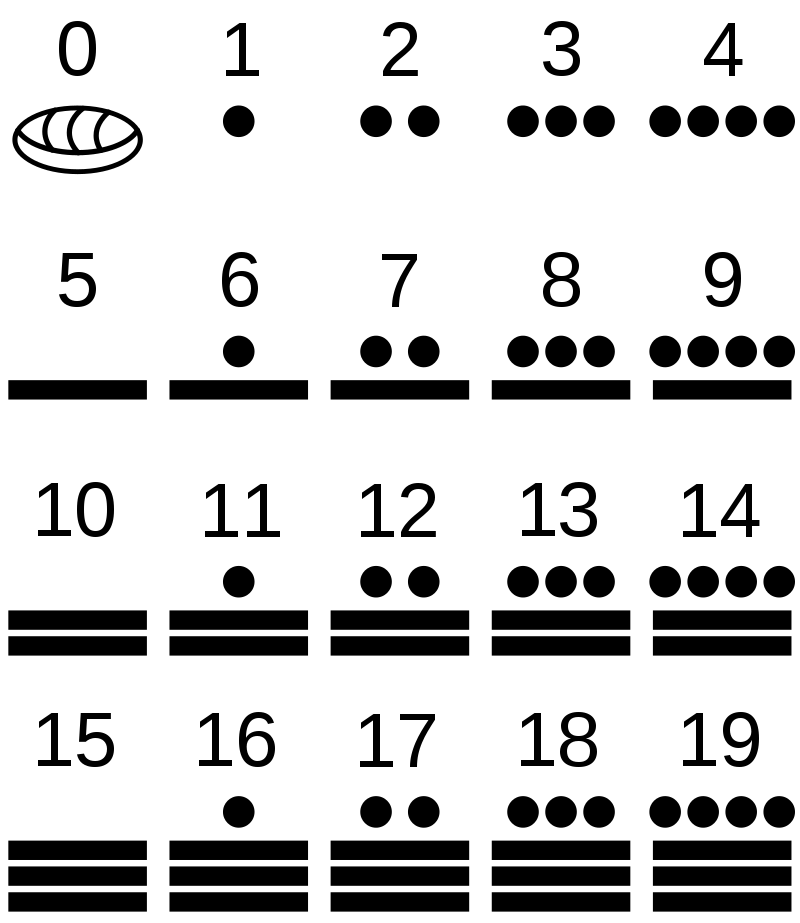
\includegraphics[width=0.2\textwidth]{figures/maya_digits.png}
\caption{\label{fig:digits} A list of the numerical digits used by the Maya.}
\end{figure}
\begin{enumerate}
\item Work out the following addition problems \textit{using the Mayan system.}
\begin{enumerate}
\item $80 + 20 = $ \vspace{2cm}
\item $365 + 365 = $ \vspace{2cm}
\item $1024 + 512 = $ \vspace{2cm}
\end{enumerate}
\item Work out the following subtraction problems \textit{using the Mayan system.}
\begin{enumerate}
\item $1024 - 512 = $ \vspace{2cm}
\item $92 - 31 = $ \vspace{2cm}
\end{enumerate}
\item Work out the following addition problems \textit{using the Incan quipu:}
\begin{enumerate}
\item $512 + 256 = $ \vspace{2cm}
\item $11 + 89 = $ \vspace{2cm}
\end{enumerate}
\item Work out the following subtraction problems \textit{using the Incan quipu:}
\begin{enumerate}
\item $365 - 67 = $ \vspace{2cm}
\item $1024 - 512 = $ \vspace{2cm}
\end{enumerate}
\item Suppose you have three terrace plots in the Andean mountains to use to survive.  You and your cohort of fellow Incans decide to grow potatoes and quinoa. Quinoa actually do better at higher altitudes that potatoes.  So the plan is to use the two lowest terraces for potatoes, and the upper four for quinoa.  Each terrace is 30 meters by 5 meters.  A potato plant requires a 0.2 meter by 0.2 meter patch, and a quinoa plant requires a 0.3 meter by 0.3 meter patch.  How many potato plants and how many quinoa plants can you plant? Store the results in a diagram of quipu knot system. \\ \vspace{2.5cm}
\end{enumerate}

\section{Connection to Physics}

\begin{figure}
\centering
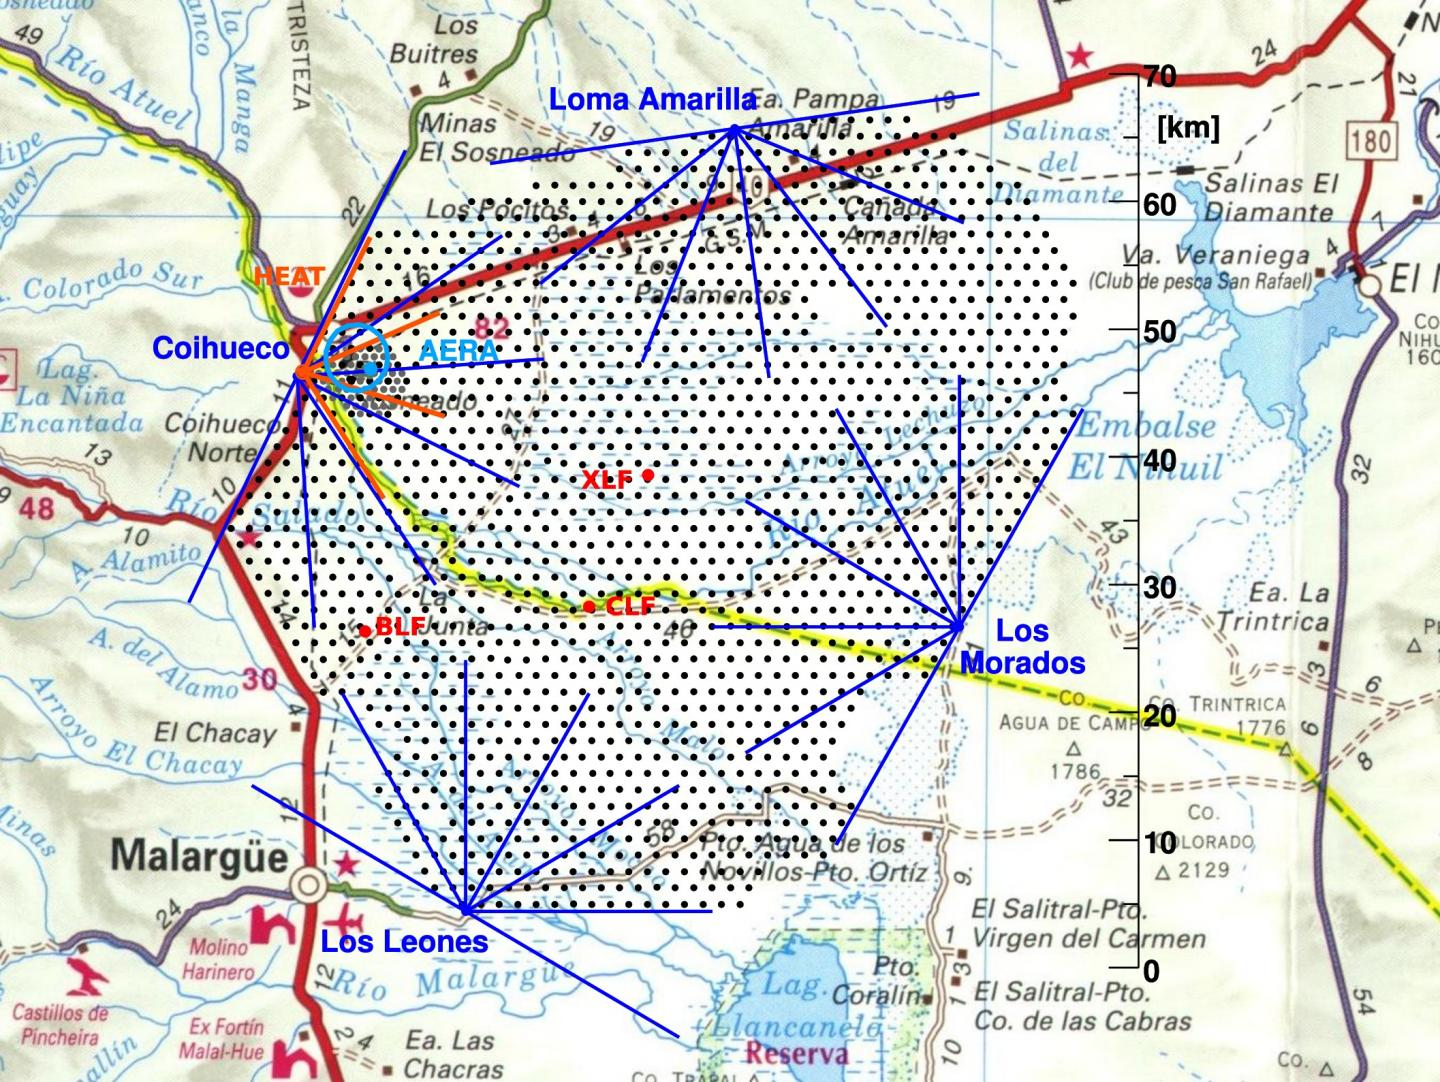
\includegraphics[width=0.5\textwidth]{figures/pao.jpg}
\caption{\label{fig:auger} A physics detector near Malarg\"{u}e, Argentina.}
\end{figure}

\begin{enumerate}
\item In Fig. \ref{fig:auger}, what physics detector is shown?
\begin{itemize}
\item A: The Large Hadron Collider
\item B: The IceCube Neutrino detector
\item C: The Pierre Auger Observatory
\item D: The High Altitude Water Cherenkov detector
\end{itemize}
\item What is the purpose of the physics project shown in Fig. \ref{fig:auger}?
\begin{itemize}
\item A: To collide protons and nuclei to probe sub-atomic physics
\item B: To detect signals from neutrinos that originate outside the solar system
\item C: To detect cosmic rays that originate outside the solar system
\item D: To detect gamma rays from space
\end{itemize}
\item What is a gamma ray?
\begin{itemize}
\item A: A photon of light
\item B: A proton or nucleus from deep space
\item C: A portion of the aurora borealis
\item D: An ion floating in the atmosphere
\end{itemize}
\item What is located at each black dot in Fig. \ref{fig:auger}? 
\begin{itemize}
\item A: A water tank designed to record Cherenkov radiation
\item B: A radio receiver designed to record radio pulses
\item C: An optical sensor designed to record visible light
\item D: A telescope designed to detect infrared radiation
\end{itemize}
\end{enumerate}

\section{Vocabulary}

\begin{enumerate}
\item What is the meaning of the term \textit{rationalism?}
\begin{itemize}
\item A: The idea that reason rather than experience is the foundation of certainty in knowledge
\item B: Encapsulating the idea of \textit{I think, therefore I am.}
\item C: Using scientific instruments
\item D: Relying on measurements and sensory experience to discover the truth
\end{itemize}
\item What is the meaning of the \textit{Nahuatl} term \textit{abuizotl?}
\begin{itemize}
\item A: A horse
\item B: A hummingbird
\item C: An otter
\item D: An alligator
\end{itemize}
\item What is the meaning of the \textit{Nahuatl} term \textit{tomatl?}
\begin{itemize}
\item A: Smoked fish
\item B: Smoked chili
\item C: An herb to help digestion
\item D: A tomato
\end{itemize}
\item What is \textit{cinchona?}
\begin{itemize}
\item A: An herb used to treat indigestion
\item B: A shrub or tree used to create quinine
\item C: A flower used in religious rituals of the \textit{Mexica} people
\item D: A plant that can form a treatment for syphilis
\end{itemize}
\item Define the word \textit{torpor}, as it pertains to animal behavior.
\begin{itemize}
\item A: The ability hover in midair during flight using rapid wingbeats
\item B: Lowering internal body temperature and metabolism to levels that render the individual immobile and in a hibernating state
\item C: The ability to break open the shells of mollusks using tools
\item D: The ability to distinguish complex sounds in songs or calls
\end{itemize}
\item Who were the \textit{Jesuits}?
\begin{itemize}
\item A: Formally known as the Order of Preachers, this is a Catholic order founded by Saint Dominic
\item B: Formally known as the Order of Friars Minor, this is a Catholic order founded by Saint Francis
\item C: Formally known as \textit{Los Amigos del Pa\'{i}s}, these were mining officials who formed guids to further economic interests of their region
\item D: Formally known as the Society of Jesus, this is a Catholic order founded by Saint Ignatius of Loyola
\end{itemize}
\end{enumerate}

\section{Free Response Section}

\begin{enumerate}
\item \textbf{Kepler's Laws, and Newtonian Physics} Discuss the varying levels of acceptance within scientific and academic communities in Nueva Granada and Per\'{u} in the late 18th century. \\ \vspace{3cm}
\item \textbf{The aurora of 1789} Discuss the significance of the aurora borealis in 1789 that was visible from Mexico City.  List several researchers who made observations of this aurora and other auroras, and explain what they found. \\ \vspace{3cm}
\item \textbf{Herbal medicine in the 16th century} Give several examples of treatments for various ailments in the body used by Europeans and indigenous Latin Americans in the 16th century.  Explain the theory of the four humors and why this influenced the European treatments but not the indigenous ones. \\ \vspace{3cm}
\item \textbf{The Inquisition, the Catholic Church, and Scientific Traditions} Discuss several examples of the following: (a) Catholic censorship of knowledge flowing from Europe to Latin America (b) Catholic censorship of knowledge flowing from Latin America to Europe (c) contributions to Latin American science by Catholic scholars and explorers (d) knowledge that was recorded or translated from indigenous sources by Catholic priests, monks, or nuns.
\end{enumerate}

\end{document}
